\documentclass{article}
\usepackage[utf8]{inputenc}
\usepackage{titling}
\usepackage{graphicx}
\usepackage{xcolor}
\usepackage[colorlinks=true,linkcolor=darkgray, urlcolor =gray]{hyperref}
\usepackage[spanish]{babel}
\DeclareUnicodeCharacter{301}{~}
\usepackage{url}
\DeclareUnicodeCharacter{202F}{\,}


\title{Programación Bluetooth con AppInventor}
\author{Cristina Díaz García}
\date{Noviembre 2018}

\renewcommand\maketitlehooka{\null\mbox{}\vfill}
\renewcommand\maketitlehookd{\vfill\null}


\begin{document}

\addcontentsline{toc}{section}{Índice general}

\begin{titlingpage}
\maketitle

\begin{center}

\includegraphics[scale=0.5]{imagenes/AppInventor.jpg} 
\end{center}

\end{titlingpage}

\newpage

\tableofcontents

\newpage

\section{Pantalla Inicial}

En la pantalla inicial tenemos dos botones, con los que iniciar el servidor o conectarse a uno ya iniciado. 

\begin{flushleft}
	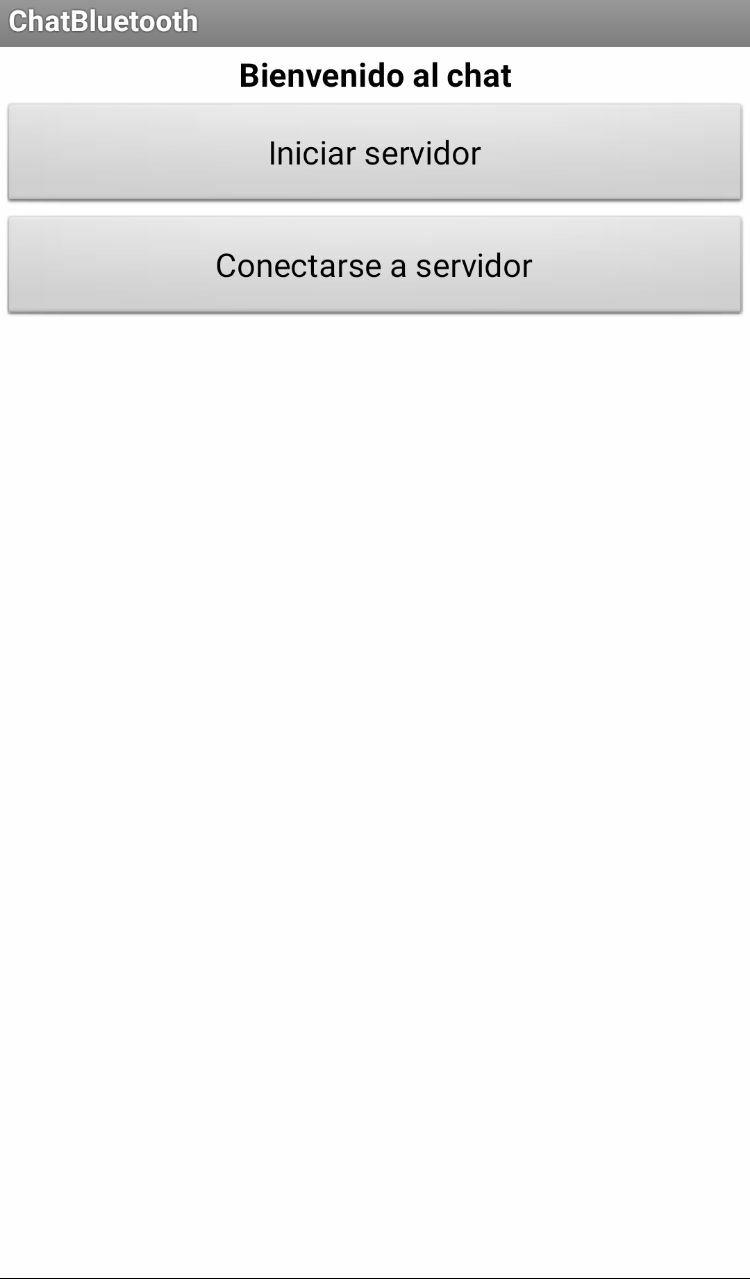
\includegraphics[scale=0.3]{imagenes/Screen1.jpg} 
\end{flushleft}

\section{Pantalla del Cliente}

En la pantalla del cliente tenemos dos botones en la cabecera, con los que conectarse y desconectarse, respectivamente. Al tocar conectar, nos saldrá una lista de los dispositivos con los que podemos conectarnos.

Debajo de estos botones, tenemos el estado de la conexión, que por defecto es \textit{desconectado}.

En la parte de abajo de la pantalla hay una caja de texto en la que podremos escribir el mensaje que queramos escribir, y a su lado hay un botón con el que enviarlo.

Debajo del estado tenemos una pantalla en la que saldrá la conversación que se está teniendo, en la que sale \textit{Yo} para los mensajes enviados y \textit{Servidor} para los mensajes recibidos.

\begin{flushleft}
	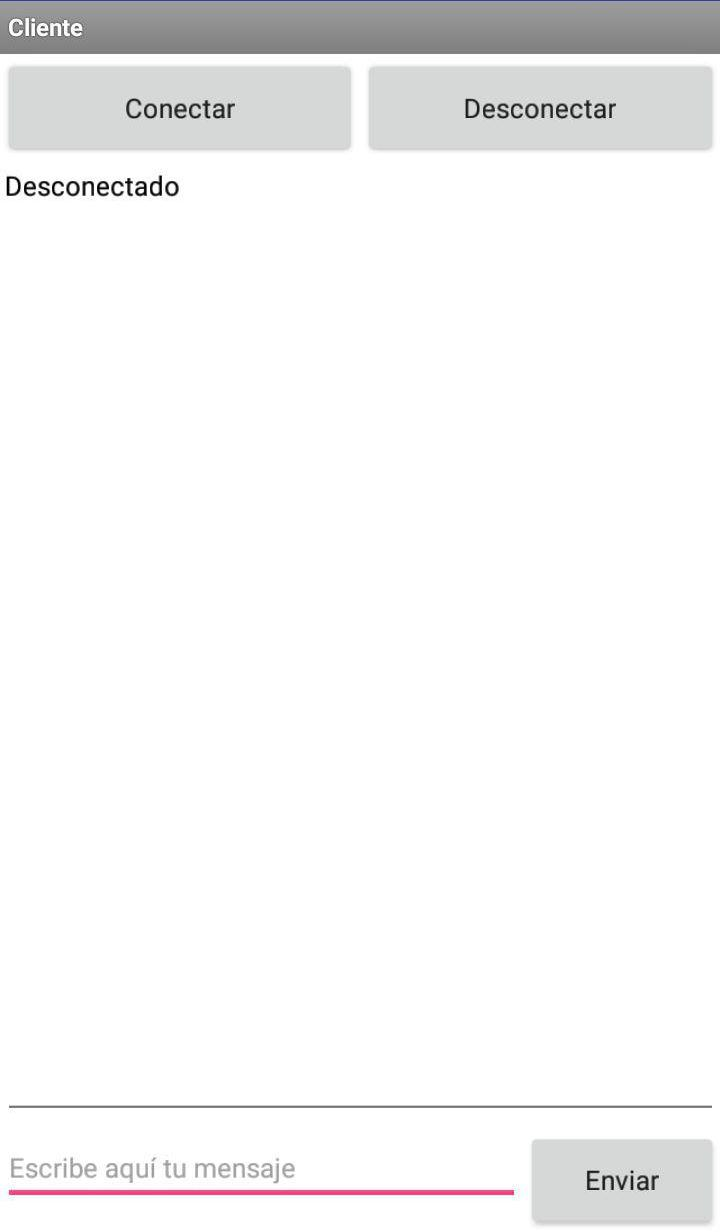
\includegraphics[scale=0.3]{imagenes/ClientePantalla.jpg} 
\end{flushleft}

Los bloques quedarían así:

\begin{flushleft}
	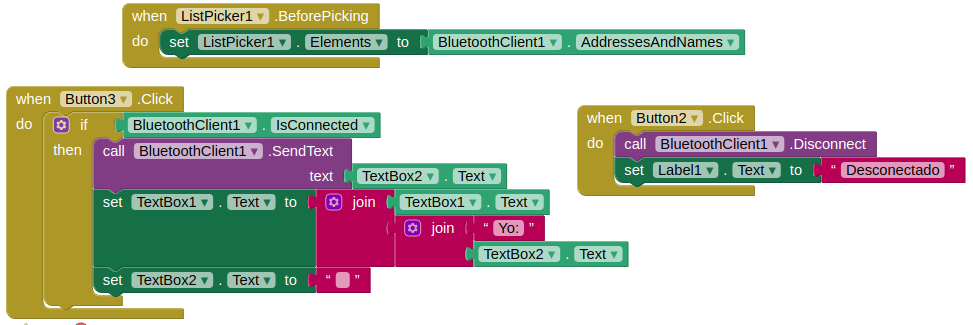
\includegraphics[scale=0.4]{imagenes/Cliente1.png} 
	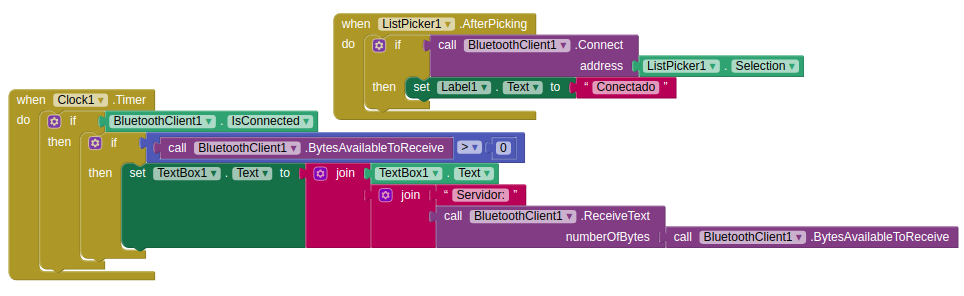
\includegraphics[scale=0.4]{imagenes/Cliente2.png} 
\end{flushleft}

Esta pantalla tiene, a mi parecer, unos cuantos problemas de implementación que no he sabido arreglar, y son:
\begin{itemize}
	\item Se puede editar la pantalla de texto de la conversación.
	\item Se pueden ``enviar`` mensajes aunque no haya conexión (no se envían por Bluetooth, pero sí al chat)
\end{itemize}

Lo intenté arreglar con estos bloques:

\begin{flushleft}
	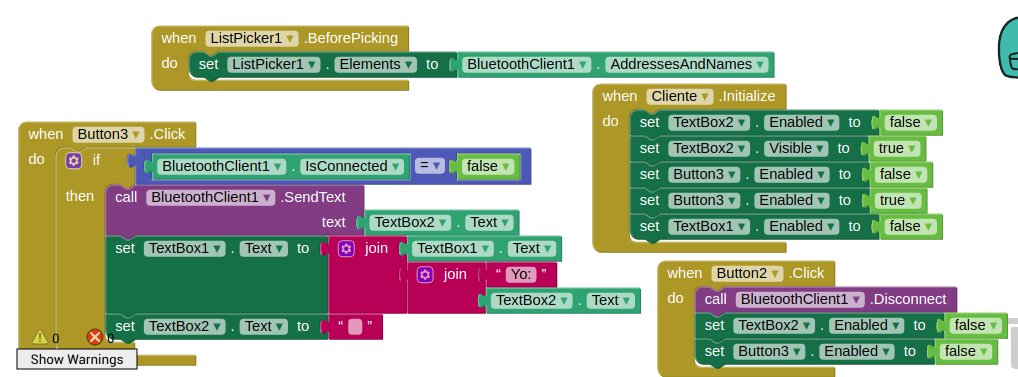
\includegraphics[scale=0.4]{imagenes/Cliente_1.png} 
	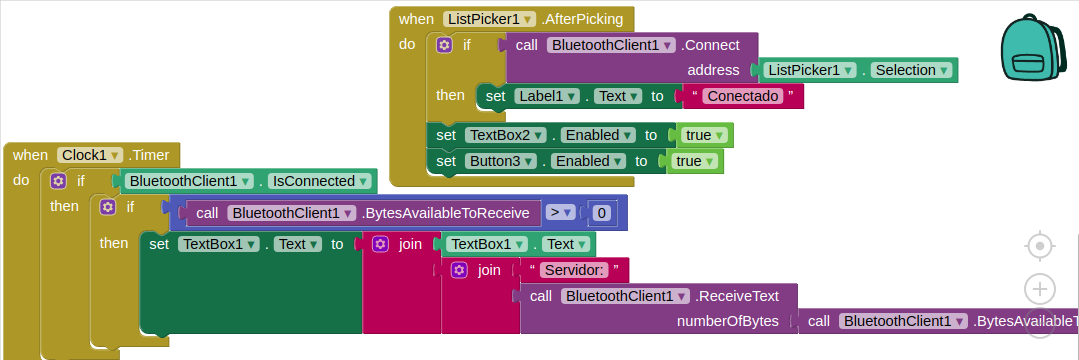
\includegraphics[scale=0.4]{imagenes/Cliente_2.png} 
\end{flushleft}

Y me dio fallos de poder editarlos aun así, no poder enviar mensajes cuando en teoría sí se debería poder o que no aparezcan las cajas de texto de abajo del todo.

\begin{flushleft}
	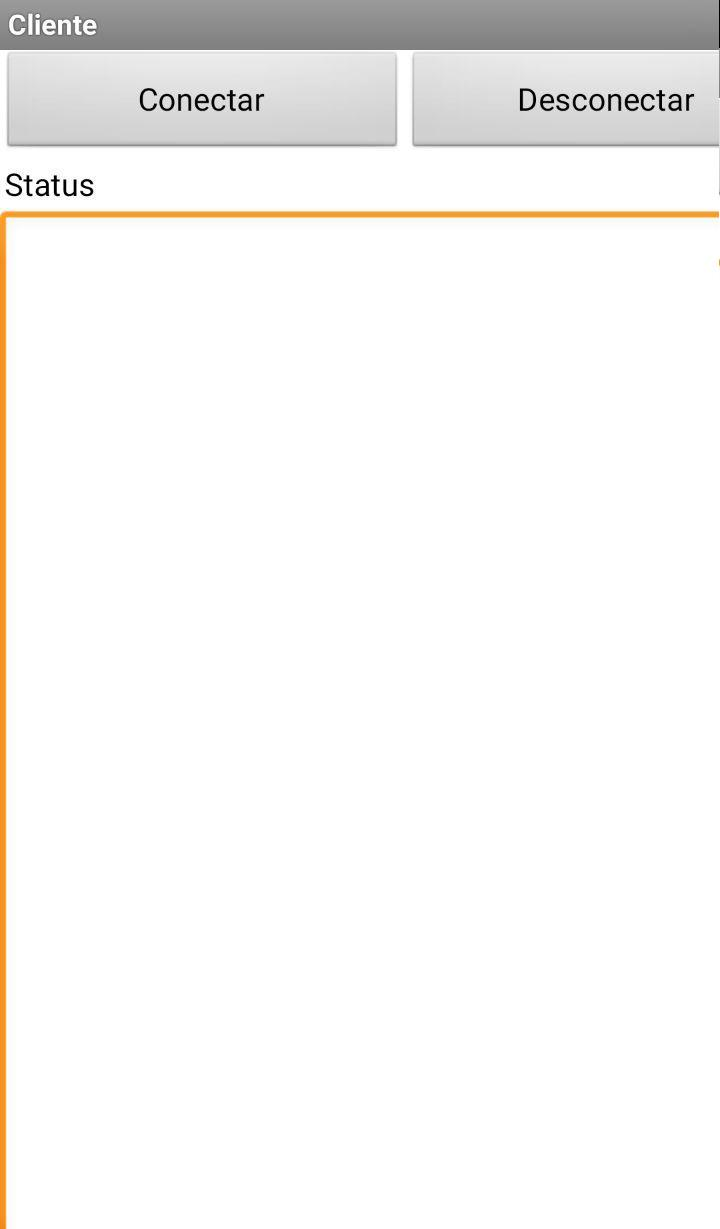
\includegraphics[scale=0.3]{imagenes/CFallo.jpg} 
\end{flushleft}

\section{Pantalla del Servidor}

En la pantalla del servidor tenemos un botón para desconectar el servidor (que nos lleva a la pantalla inicial), una caja de texto con la conversación, una caja de texto para el mensaje que queramos enviar y un botón para hacerlo.

\begin{flushleft}
	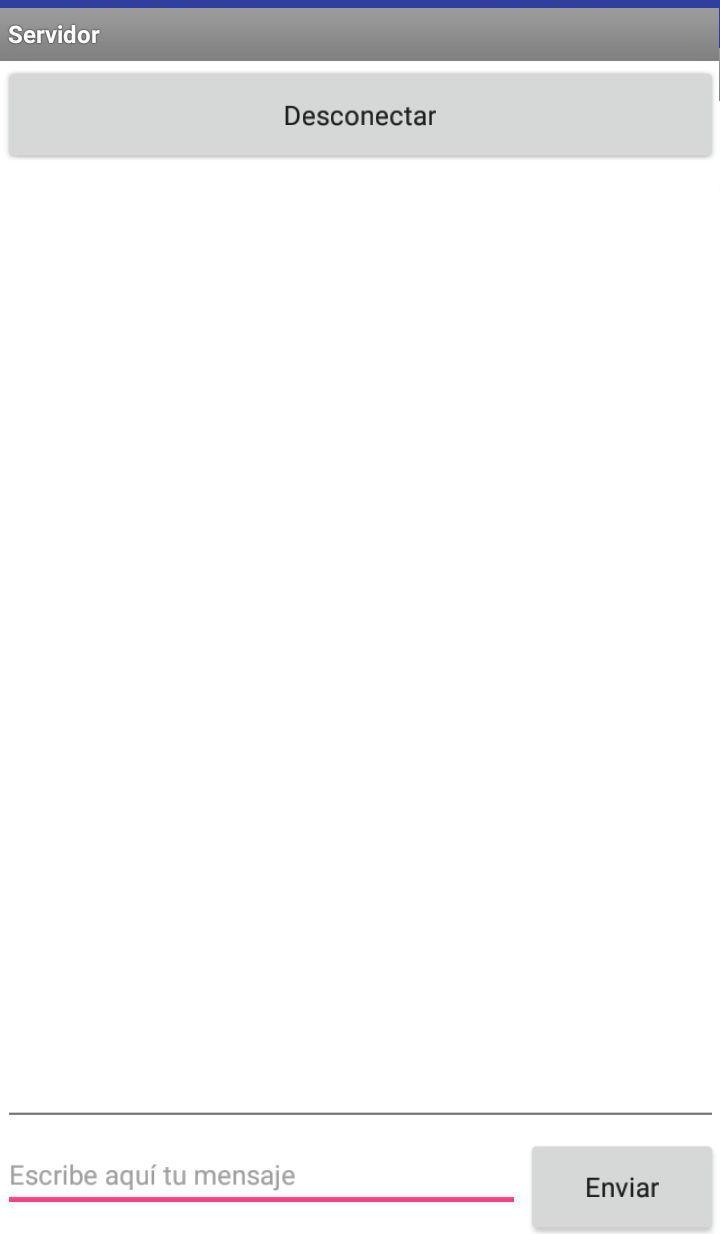
\includegraphics[scale=0.3]{imagenes/ServidorPantalla.jpg} 
\end{flushleft}

Los bloques quedarían así:

\begin{flushleft}
	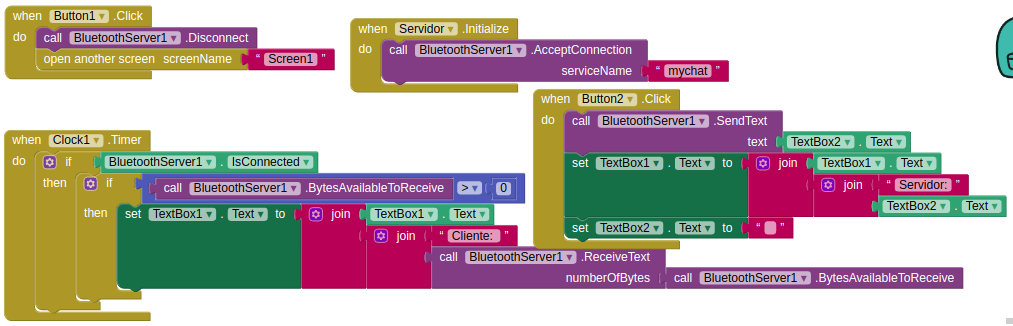
\includegraphics[scale=0.4]{imagenes/Servidor.png} 
\end{flushleft}

Al igual que en el cliente, los fallos que veo son que hay bloques de texto que no deberían ser editables y lo son. Lo inteneté solventar con los siguientes bloques:

\begin{flushleft}
	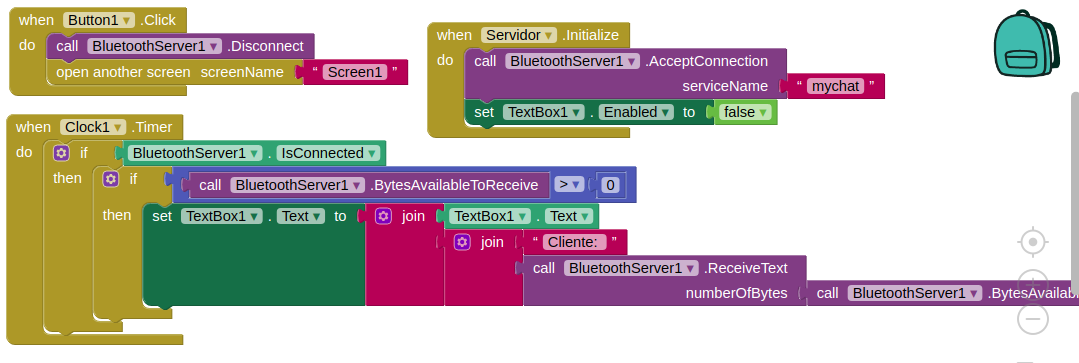
\includegraphics[scale=0.4]{imagenes/Servidor_1.png} 
	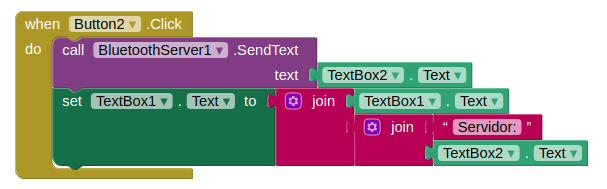
\includegraphics[scale=0.4]{imagenes/Servidor_2.png} 
\end{flushleft}

Y me daba los mismos problemas que en el cliente:

\begin{flushleft}
	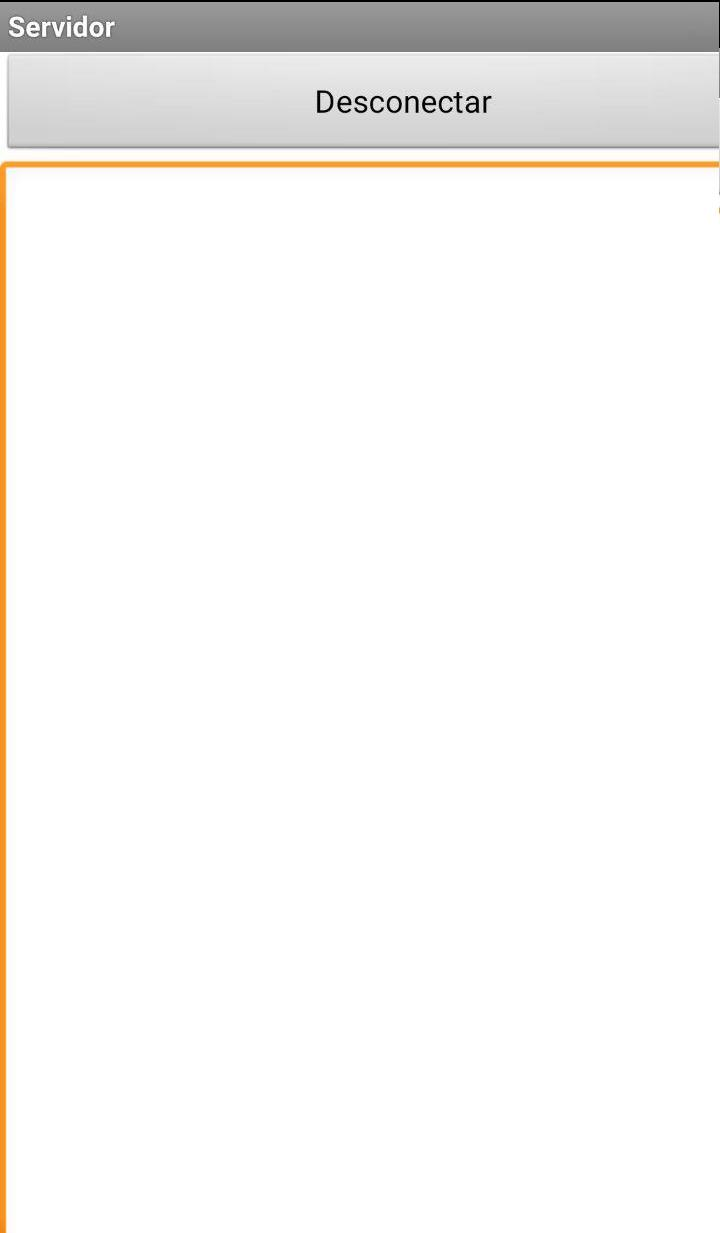
\includegraphics[scale=0.2]{imagenes/SFallo.jpg} 
\end{flushleft}

\section{COMUNICACIÓN CLIENTE-SERVIDOR}

Esta es la vista desde el cliente:

\begin{flushleft}
	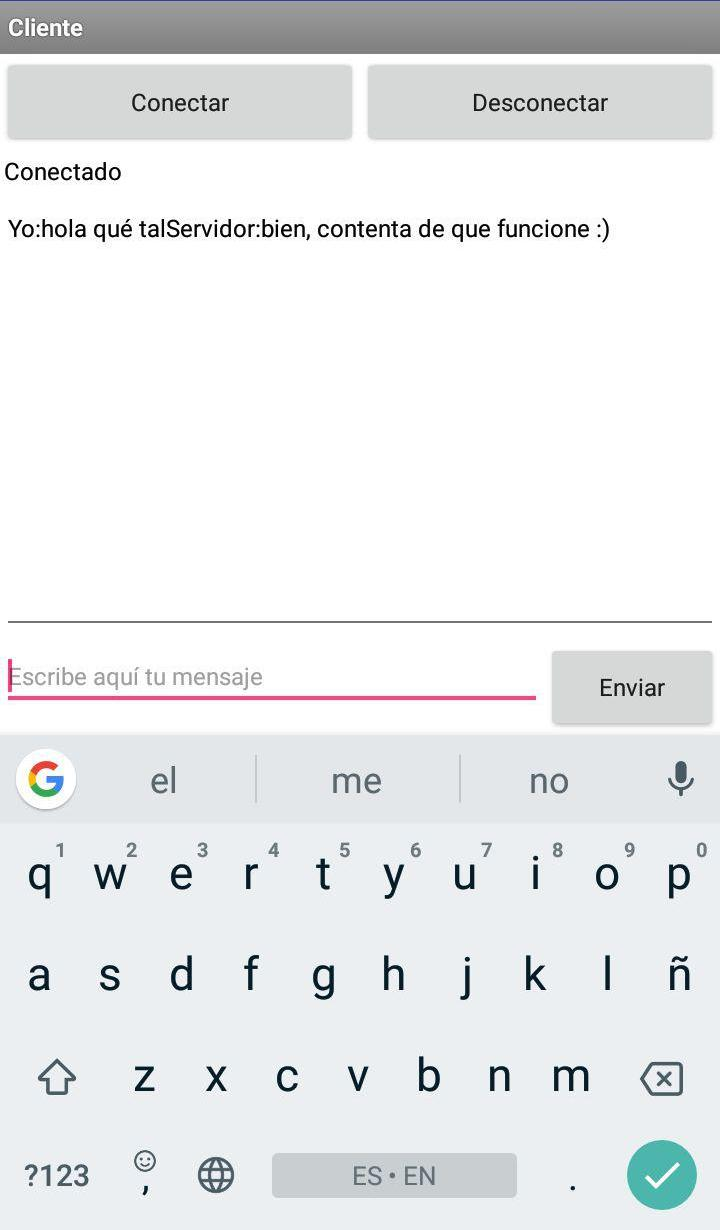
\includegraphics[scale=0.2]{imagenes/ChatClient.jpg} 
\end{flushleft}

Y esta es la vista desde el servidor:

\begin{flushleft}
	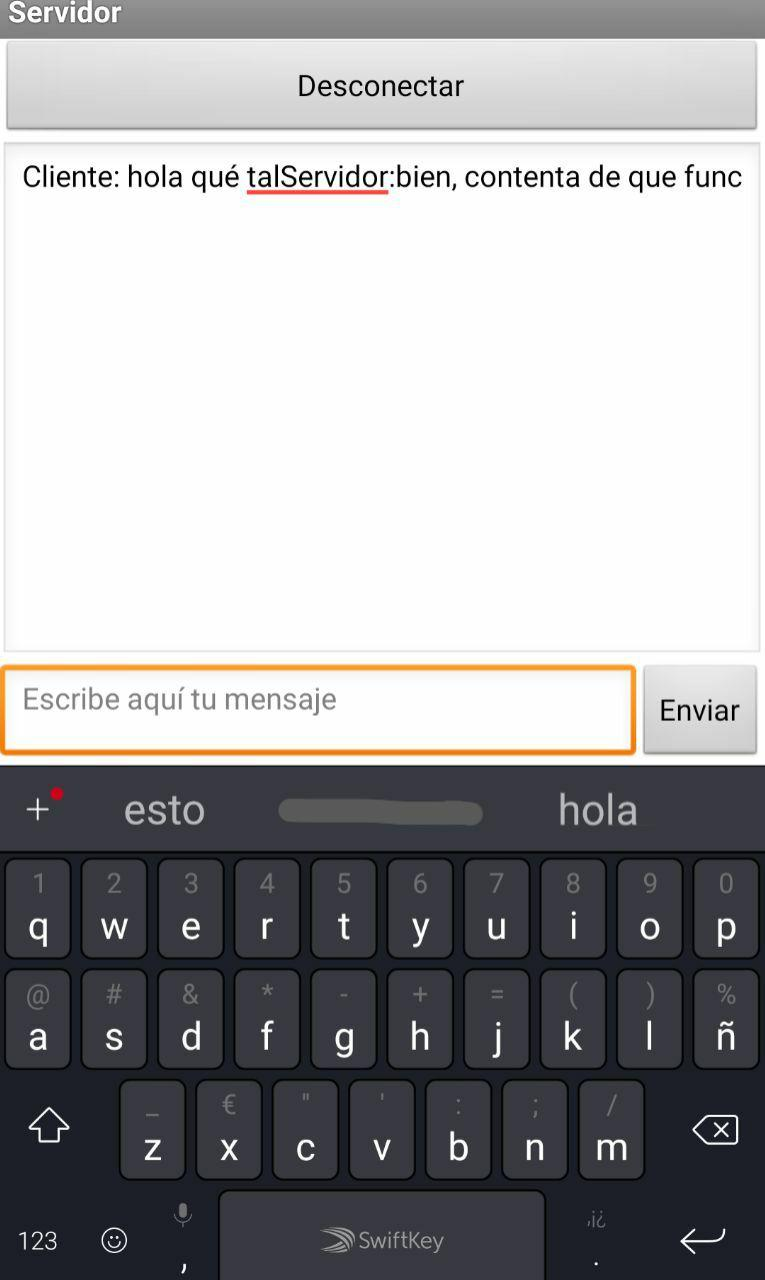
\includegraphics[scale=0.2]{imagenes/ChatServ.jpg} 
\end{flushleft}

Como se puede ver, otro de los fallos existentes es que los mensajes no saltan de línea al escribirse.

\end{document}